\chapter{Boundary operator}
\label{chapter:boundary-operator}

In this chapter we present the boundary operator defined in the theory of discrete calculus and we propose a curvature-based model using this concept.

\section{Cellular grid model}

We restrict our analysis to the integer plan because it's where theory and application is developped in this thesis, but it can be extended to higher dimensions. In the plan $\mathbb{Z}^2$, we identify faces (pixels), edges (linels) and vertices (pointels). An arbitrary (however coherent) orientation is set for faces and edges. For example, we set faces counter-clockwise, vertical edges to point up and horizontal edges to point right (see figure).

\begin{definition}{Boundary operator}
	Let $\Omega \in \mathbb{Z}^2$ be a connected portion of the integer plan with $m$ faces and $n$ edges. The boundary operator $\partial \in \mathbb{Z}^{n \times m}$ is a matrix in which each column $\partial _j$ represents the incidence relations between face $j$ and the edges of the domain.
\end{definition}

A face is incident to an edge if the edge itself is part of the face's boundary and not incident otherwise. We say it is positive incident to an edge if besides incident, the face orientation  agrees with the orientation the edge, and negative incident in the case it doesn't agree.

\[
\partial _{i,j} = \left\{ \begin{array}{ll}
	1, & \text{face $j$ is positive incident to edge $i$}\\
	-1, & \text{face $j$ is negative incident to edge $i$}\\	
	0, & \text{otherwise}
\end{array}\right.
\]

\begin{example}
	Consider a portion $\Omega$ of $\mathbb{Z}^2$ with $9$ faces ,$24$ edges and orientation as depicted in figures \ref{fig:cell-grid-indices} and \ref{fig:cell-grid-orientation}. 	
	
\begin{figure}[h!]
\center
\subfloat[\label{fig:cell-grid-indices}]{%
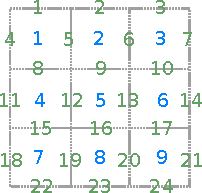
\includegraphics[scale=1]{figures/appendix-boundary-operator/cell-grid-1.pdf}}\hspace{1em}%
\subfloat[\label{fig:cell-grid-orientation}]{%
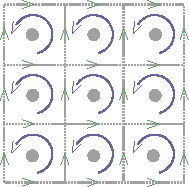
\includegraphics[scale=1]{figures/appendix-boundary-operator/cell-grid-2.pdf}}\hspace{1em}%
\subfloat[\label{fig:cell-grid-active-pixels}]{%
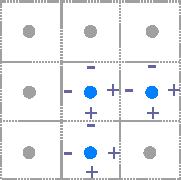
\includegraphics[scale=1]{figures/appendix-boundary-operator/cell-grid-3.pdf}}\hspace{1em}%
\subfloat[\label{fig:cell-grid-active-linels}]{%
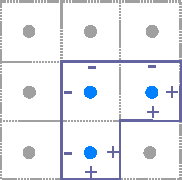
\includegraphics[scale=1]{figures/appendix-boundary-operator/cell-grid-4.pdf}}%
\caption{Figures (a) and (b) illustrates indices assignments and orientation; figure (d) shows the result of applying the boundary operator for the active pixels in figure (c).}
\end{figure}

\[
   \begin{array}{ll}
	
	\partial = \left[ \begin{array}{ccccccccc}
	 -1 & 0 & 0 & 0 & 0 & 0 & 0 & 0 & 0 \\
	 0 & -1 & 0 & 0 & 0 & 0 & 0 & 0 & 0 \\	 
	 0 & 0 & -1 & 0 & 0 & 0 & 0 & 0 & 0 \\	 
	 -1 & 0 & 0 & 0 & 0 & 0 & 0 & 0 & 0 \\	 
	 1 & -1 & 0 & 0 & 0 & 0 & 0 & 0 & 0 \\	 
	 0 & 1 & -1 & 0 & 0 & 0 & 0 & 0 & 0 \\	 
	 0 & 0 & 1 & 0 & 0 & 0 & 0 & 0 & 0 \\	 
	 1 & 0 & 0 & -1 & 0 & 0 & 0 & 0 & 0 \\	 
	 0 & 1 & 0 & 0 & -1 & 0 & 0 & 0 & 0 \\	 
	 0 & 0 & 1 & 0 & 0 & -1 & 0 & 0 & 0 \\	 
	 0 & 0 & 0 & -1 & 0 & 0 & 0 & 0 & 0 \\	 
	 0 & 0 & 0 & 1 & -1 & 0 & 0 & 0 & 0 \\	 
	 0 & 0 & 0 & 0 & 1 & -1 & 0 & 0 & 0 \\	 
	 0 & 0 & 0 & 0 & 0 & 1 & 0 & 0 & 0 \\	 
	 0 & 0 & 0 & 1 & 0 & 0 & -1 & 0 & 0 \\	 
	 0 & 0 & 0 & 0 & 1 & 0 & 0 & -1 & 0 \\	 
	 0 & 0 & 0 & 0 & 0 & 1 & 0 & 0 & -1 \\	 
	 0 & 0 & 0 & 0 & 0 & 0 & -1 & 0 & 0 \\	 
	 0 & 0 & 0 & 0 & 0 & 0 & 1 & -1 & 0 \\	 
	 0 & 0 & 0 & 0 & 0 & 0 & 0 & 1 & -1 \\	 
	 0 & 0 & 0 & 0 & 0 & 0 & 0 & 0 & 1 \\	 
	 0 & 0 & 0 & 0 & 0 & 0 & 1 & 0 & 0 \\	 
	 0 & 0 & 0 & 0 & 0 & 0 & 0 & 1 & 0 \\	 
	 0 & 0 & 0 & 0 & 0 & 0 & 0 & 0 & 1	 	 	 	 	 	 	 		\end{array}\right] &, \qquad
	 
	\partial \left[ \begin{array}{l}
					0\\
					0\\
					0\\
					0\\
					1\\
					1\\
					0\\
					1\\
					0\\
					\end{array}\right] =  \left[ \begin{array}{l}
											0\\
											0\\
											0\\
											0\\
											0\\
											0\\
											0\\
											0\\
											-1\\
											-1\\
											0\\
											-1\\
											0\\
											1\\
											0\\
											0\\
											1\\
											0\\
											-1\\
											1\\
											0\\
											0\\
											1\\
											0
										\end{array}\right]
	 
   \end{array}
\]



The boundary operator applied for vector $x \in \mathbb{Z}^9$, representing the active pixels depicted in figure \ref{fig:cell-grid-active-pixels}, results in vector $y \in \mathbb{Z}^{24}$ representing the active boundary depicted in figure \ref{fig:cell-grid-active-linels}.

The coboundary operator is simply defined as the transpose of the boundary operator. The coboundary operator applied to a vector of active linels returns the set of incident pixels to the linels. For example, $\partial^{T}\partial$ applied to vector $x$ above results in $[0,-1,-1,-1,2,3,-1,3,-2]^T$. Positive coefficients represents inner incident pixels, and negative coefficients outer incident pixels. Moreover, the absolute value of each coefficient represents the number of linels incident to the corresponding pixel. For example, pixel $6$ is incident to three linels, namely the linels $10,14,17$.

\end{example}

\section{Squared Curvature Model}

Let $\Omega \in \mathbb{Z}^2$ be a portion of the integer plane with $m$ pixels and $n$ linels. For a given euclidean shape $S$, we assume that its digitization $D$ is embeded in $\Omega$. We wish to evolve $D$ to a digital shape $D^\prime$ such that $E(D^\prime) < E(D)$.

We partition $\Omega$ in sets $X,F,B$ representing the optimization, foreground and background domains. Vectors $\mathbbm{1}_X, \mathbbm{1}_F, \mathbbm{1}_B \in \mathbb{B}^m$ represent its respective active vectors.

\begin{example}
	The pixel incidence vector $q \in \mathbb{Z}^m$ for initial digital shape $D$ is given by
	
	\begin{align*}
		q &= \partial^T\partial (\mathbbm{1}_X + \mathbbm{1}_F)\\
		&=\partial^T\partial (\mathbbm{1}_X) + \partial^T\partial (\mathbbm{1}_F)\\ 
		&= q_X + q_F
	\end{align*}
\end{example}

For a given vector $x \in \mathbb{Z}^k$, we define its matrix filter $\hat{x} \in \mathbb{Z}^{k\times k}$ as

\[
	\hat{x}_{i,j} = \left\{ \begin{array}{ll}
	1, & i=j \text{ and } x_i \neq 0 \\
	0, & \text{otherwise}.
	\end{array}\right.
\]

Let $B \in \mathbb{B}^{m\times m}$ such that column vector $B_i$ represents the pixels in the interior of a disk of radius $R$ centered at pixel $i$. Finally, we define the energy as

\begin{align*}
	E = \frac{9}{R^6}\frac{1}{4}\sum_{i}^{m}{\left( \frac{\pi R^2}{2} - x^T\hat{q_X}B_ix_i - q_F^TB_i \right)^2}.
\end{align*}

The $0.25$ factor is due to the estimation ball computation on both incident pixels for each linel. We set a factor of $0.5$ for each ball, that becomes $0.25$ when powered to the square. 

Energy $E$ is of fourth order. If we relax variable $x$ to its real counterpat, a local optima for the relaxed problem is such that each coefficient of its gradient equals to zero. Therefore, if we know how to find the roots of the $m$ gradient coeffients expressions, we are done.

Notice that we recover $JMIV$ energy if we consider the minimization in a fixed contour, namely the contour of the original digital shape $D$.

\begin{align*}
	E_{JMIV} = \frac{9}{R^6}\frac{1}{4}\sum_{i}^{m}{\left( \frac{\pi R^2}{2} - x^T\hat{q_X}B_i - q_F^TB_i \right)^2}.
\end{align*}

\section{Numerical methods}

\begin{itemize}
	\item{Newton-Rapson}
	\item{Homotopy Continuation Method (Hom4PS-3)}
\end{itemize}


